% Generated by ICLR_Q4.py from experiment_logs_Q4 -- Dubins4D_x0set: Reach-avoid prob.
% Shaded band = min/max over seeds; line = median over seeds.
% Picture width is exactly \linewidth. Requires \usepackage{pgfplots}.
% Broken y axis: 0-0.9 fills the bottom half of the plot, 0.9-1 the top half.
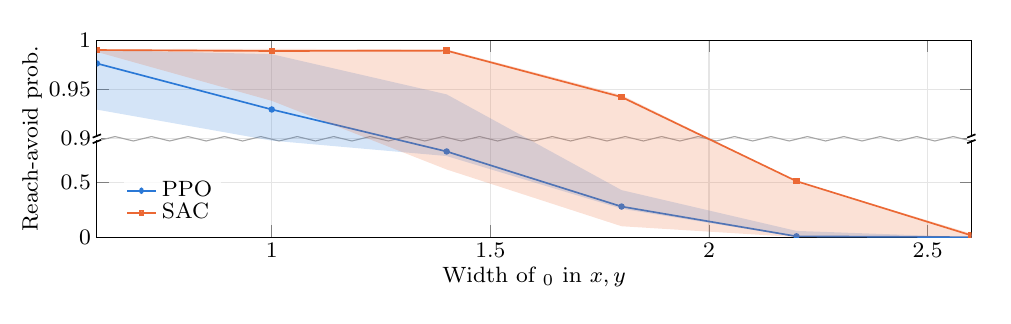
\begin{tikzpicture}[baseline=(current axis.south)]
\definecolor{q4ppo}{RGB}{42,120,214}
\definecolor{q4sac}{RGB}{235,104,52}
\begin{axis}[
    scale only axis, width=\linewidth-25pt-4pt, height=2.5cm,
    xlabel={Width of $\X_0$ in $x,y$},
    ylabel={Reach-avoid prob.}, ylabel style={align=center},
    xmin=0.6, xmax=2.6, xtick={1,1.5,2,2.5},
    ymin=0, ymax=1, ytick={0,0.5,0.9,0.95,1}, yticklabels={0,0.5,0.9,0.95,1},
    grid=major, grid style={gray!20}, clip marker paths=true,
    label style={font=\footnotesize}, tick label style={font=\footnotesize, inner sep=2pt},
    xlabel shift=-2pt, ylabel shift=-3pt,  % labels close to the tick labels
    y coord trafo/.code={\pgfmathparse{#1 < 0.9 ? #1*0.555556 : 0.5 + (#1 - 0.9)*5}},
    y coord inv trafo/.code={\pgfmathparse{#1 < 0.5 ? #1/0.555556 : 0.9 + (#1 - 0.5)/5}},
    legend pos=south west, legend cell align=left,
    legend style={font=\footnotesize, draw=none, fill=white, fill opacity=0.8, text opacity=1,
        inner sep=1pt, row sep=-3pt},
    legend image post style={xscale=0.6},
]
% Zigzag line across the plot at 0.9, where the y scale changes (drawn below the data)
\draw[gray!70, thin, line join=round] ([yshift=-0.8pt]rel axis cs:0,0.5) -- ([yshift=0.8pt]rel axis cs:0.02083,0.5) -- ([yshift=-0.8pt]rel axis cs:0.04167,0.5) -- ([yshift=0.8pt]rel axis cs:0.0625,0.5) -- ([yshift=-0.8pt]rel axis cs:0.08333,0.5) -- ([yshift=0.8pt]rel axis cs:0.1042,0.5) -- ([yshift=-0.8pt]rel axis cs:0.125,0.5) -- ([yshift=0.8pt]rel axis cs:0.1458,0.5) -- ([yshift=-0.8pt]rel axis cs:0.1667,0.5) -- ([yshift=0.8pt]rel axis cs:0.1875,0.5) -- ([yshift=-0.8pt]rel axis cs:0.2083,0.5) -- ([yshift=0.8pt]rel axis cs:0.2292,0.5) -- ([yshift=-0.8pt]rel axis cs:0.25,0.5) -- ([yshift=0.8pt]rel axis cs:0.2708,0.5) -- ([yshift=-0.8pt]rel axis cs:0.2917,0.5) -- ([yshift=0.8pt]rel axis cs:0.3125,0.5) -- ([yshift=-0.8pt]rel axis cs:0.3333,0.5) -- ([yshift=0.8pt]rel axis cs:0.3542,0.5) -- ([yshift=-0.8pt]rel axis cs:0.375,0.5) -- ([yshift=0.8pt]rel axis cs:0.3958,0.5) -- ([yshift=-0.8pt]rel axis cs:0.4167,0.5) -- ([yshift=0.8pt]rel axis cs:0.4375,0.5) -- ([yshift=-0.8pt]rel axis cs:0.4583,0.5) -- ([yshift=0.8pt]rel axis cs:0.4792,0.5) -- ([yshift=-0.8pt]rel axis cs:0.5,0.5) -- ([yshift=0.8pt]rel axis cs:0.5208,0.5) -- ([yshift=-0.8pt]rel axis cs:0.5417,0.5) -- ([yshift=0.8pt]rel axis cs:0.5625,0.5) -- ([yshift=-0.8pt]rel axis cs:0.5833,0.5) -- ([yshift=0.8pt]rel axis cs:0.6042,0.5) -- ([yshift=-0.8pt]rel axis cs:0.625,0.5) -- ([yshift=0.8pt]rel axis cs:0.6458,0.5) -- ([yshift=-0.8pt]rel axis cs:0.6667,0.5) -- ([yshift=0.8pt]rel axis cs:0.6875,0.5) -- ([yshift=-0.8pt]rel axis cs:0.7083,0.5) -- ([yshift=0.8pt]rel axis cs:0.7292,0.5) -- ([yshift=-0.8pt]rel axis cs:0.75,0.5) -- ([yshift=0.8pt]rel axis cs:0.7708,0.5) -- ([yshift=-0.8pt]rel axis cs:0.7917,0.5) -- ([yshift=0.8pt]rel axis cs:0.8125,0.5) -- ([yshift=-0.8pt]rel axis cs:0.8333,0.5) -- ([yshift=0.8pt]rel axis cs:0.8542,0.5) -- ([yshift=-0.8pt]rel axis cs:0.875,0.5) -- ([yshift=0.8pt]rel axis cs:0.8958,0.5) -- ([yshift=-0.8pt]rel axis cs:0.9167,0.5) -- ([yshift=0.8pt]rel axis cs:0.9375,0.5) -- ([yshift=-0.8pt]rel axis cs:0.9583,0.5) -- ([yshift=0.8pt]rel axis cs:0.9792,0.5) -- ([yshift=-0.8pt]rel axis cs:1,0.5);
% PPO: 5 seeds per X0 span
\addplot[draw=none, fill=q4ppo, fill opacity=0.2, forget plot] coordinates {(0.6,0.929625) (1,0.882996) (1.4,0.742007) (1.8,0.259818) (2.2,0.0022184) (2.6,7.25751e-08) (2.6,7.41889e-06) (2.2,0.0575252) (1.8,0.430475) (1.4,0.945096) (1,0.985959) (0.6,0.990287)} -- cycle;
\addplot[q4ppo, semithick, mark=*, mark size=0.85pt] coordinates {(0.6,0.976511) (1,0.929754) (1.4,0.783714) (1.8,0.280157) (2.2,0.00795742) (2.6,3.39054e-07)};
\addlegendentry{PPO}
% SAC: 2/5 seeds per X0 span
\addplot[draw=none, fill=q4sac, fill opacity=0.2, forget plot] coordinates {(0.6,0.988255) (1,0.938558) (1.4,0.619015) (1.8,0.100169) (2.2,0.00122616) (2.6,0) (2.6,0.0328988) (2.2,0.513128) (1.8,0.944437) (1.4,0.990815) (1,0.991339) (0.6,0.991103)} -- cycle;
\addplot[q4sac, semithick, mark=square*, mark size=0.85pt] coordinates {(0.6,0.990163) (1,0.989182) (1.4,0.989519) (1.8,0.942418) (2.2,0.512191) (2.6,0.0164494)};
\addlegendentry{SAC}
\end{axis}
% Break marks on both sides of the y axis at 0.9, where the scale changes
\path (current axis.south west) -- (current axis.north west) coordinate[pos=0.5] (q4brkW);
\path (current axis.south east) -- (current axis.north east) coordinate[pos=0.5] (q4brkE);
\foreach \p in {q4brkW, q4brkE} {
    \fill[white] ([xshift=-1.5pt, yshift=-0.6pt]\p) rectangle ([xshift=1.5pt, yshift=0.6pt]\p);
    \draw[semithick] ([xshift=-1.5pt, yshift=-1.6pt]\p) -- ([xshift=1.5pt, yshift=-0.4pt]\p)
                     ([xshift=-1.5pt, yshift=0.4pt]\p) -- ([xshift=1.5pt, yshift=1.6pt]\p);
}
% Fix the bounding box to exactly \linewidth wide: the axis box plus the label margins
\path (current axis.south west |- current bounding box.south) ++(-25pt,0) coordinate (q4sw)
      (current axis.north east |- current bounding box.north) ++(4pt,0) coordinate (q4ne);
\pgfresetboundingbox
\useasboundingbox (q4sw) rectangle (q4ne);
\end{tikzpicture}%
